\documentclass[10pt]{beamer}

\usetheme{Montpellier}
\usecolortheme{whale}

\usepackage[T1]{fontenc}
\usepackage{lmodern}

\usepackage{mathtools}
\usepackage[binary-units]{siunitx}
\usepackage{amsmath}
\usepackage{listings}
\usepackage{mdframed}
\usepackage{adjustbox}
\usepackage{minted}
\usepackage{xcolor}

\usepackage{parskip}
\usepackage{substr}
\usepackage{hyperref}
\usepackage{etoolbox}
\usepackage{tipa}
\usepackage{cprotect}
\usepackage{booktabs}
\usepackage{silence}
\usepackage[backend=biber, style=ieee]{biblatex}
\usepackage[english,ngerman]{babel}
\usepackage{csquotes}

\definecolor{lg}{gray}{0.95}
\hypersetup{colorlinks = true, urlcolor=blue, linkcolor=white}
\WarningFilter{biblatex}{Patching footnotes failed}

\renewcommand*{\bibfont}{\tiny}
\renewcommand{\subsectionname}{AA}

\bibliography{resources.bib}

\title{\textbf{Operating Systems}}
\subtitle{Tutorial 6}
\author{Fabian Klopfer}
\date{\today}

\defbeamertemplate{subsection page}{mine}[1][]{%
  \begin{centering}
    {\usebeamerfont{subsection name}\usebeamercolor[fg]{subsection name}#1}
    \vskip1em\par
    \begin{beamercolorbox}[sep=12pt,center]{part title}
      \usebeamerfont{subsection title}\insertsubsection\par
    \end{beamercolorbox}
  \end{centering}
}

\defbeamertemplate{section page}{mine}[1][]{%
  \begin{centering}
    {\usebeamerfont{section name}\usebeamercolor[fg]{section name}#1}
    \vskip1em\par
    \begin{beamercolorbox}[sep=12pt,center]{part title}
      \usebeamerfont{section title}\insertsection\par
    \end{beamercolorbox}
  \end{centering}
}

\setbeamertemplate{section page}[mine]
\setbeamertemplate{subsection page}[mine]

\begin{document}
\frame{\titlepage}


\begin{frame}{Intro}
\begin{itemize}
 \item Pingo Polls
\end{itemize}
\end{frame}

\section*{Exercise Sheet 5}
\frame{\sectionpage}
\subsection*{Exercise 1}
\frame{\subsectionpage}
\begin{frame}[allowframebreaks, fragile]{Exercise 1}
    \begin{enumerate}
		\item What problem does paging solve? \\
		\alert{\begin{itemize}
		        \item Virtual address space larger than physical
		        \item Paging splits virtual address space into chunks 
		        \item Loads them in available frames in RAM.
		       \end{itemize}
        }
		
		\item What is the difference between swapping and paging?\\
		\alert{
            \begin{itemize}
             \item Paging splits virtual address space into smaller chunks and loads them as needed. $\Rightarrow$ Small parts of processes address space.
             \item Swapping stores currently inactive processes to disk and loads them if active again. $\Rightarrow$ Complete address space of process.
            \end{itemize}
		}
		
		\item What is the difference between overlays and paging?\\
		\alert{
            \begin{itemize}
             \item Overlays: Splitting \& loading is done by hand by application programmer
             \item Paging: Splitting \& loading is done automagically by OS
            \end{itemize}

		}
		\framebreak
		\item What is a page and what is a page frame?\\
		\alert{
            \begin{itemize}
             \item Page: A chunk of  continuous virtual address space
             \item Frame: A chunk of continuous physical address space/RAM
            \end{itemize}
		}
		
		\item What is the relation between the size of pages and the size of page frames?\\
		\alert{
            Normally same size.
		}
		
		\item Why do pages usually have a size that corresponds to a power of two?\\
		\alert{
		Addressing \& Address translation in binary format/with binary ops
		}
		
		\item What is the function of page tables? \\
		\alert{
            Stores mapping from virtual pages to physical frames. \\
             Page frame address + offset = physical address
		}
		
		\item What is a page fault? \\
		\alert{
		Is what happens when page is looked up in page table \& the absent bit is set.\\
		On page fault, OS executes page fault handler to load the page from disk to frame.
		}
		
		\item What problem does segmentation solve?\\
		\alert{
		Eases MM by providing multiple separate address spaces to a process
		}
		
		\item Can paging and segmentation be combined? \\
		\alert{
		Yes e.g. Intel x86
		}
	\end{enumerate}
\end{frame}

\subsection*{Exercise 2}
\frame{\subsectionpage}
\begin{frame}[allowframebreaks, fragile]{Exercise 2}
    Two-dimensional array \mintinline{c}{int X[64][64]}, four page frames each has space for 128 values of type \mintinline{c}{int}. \\
	Calculate the number of page faults: \\
	
	\alert{
	 Array uses $\frac{64^2}{128} = \frac{(32 \cdot 2) \cdot 64}{128} = \frac{128 \cdot 32}{128} = 32$ Pages.
	 }
	 \framebreak
	 
    \begin{minted}[autogobble]{c}
    // Fragment A
    for (int j = 0; j < 64; ++j)
        for (int i = 0; i < 64; ++i)
            X[i][j] = 0;
    \end{minted}
    \alert{
    \begin{itemize}
     \item Inner loop iterates over rows, outer over columns.
     \item only two elements of page are accessed before next page needed
     \item each second access leads to a page fault
    \end{itemize}
    \[ \frac{64^2}{2} = \frac{2 \cdot 32 \cdot 64}{2} = 64 \cdot 32 = 2^6 \cdot 2^5 = 2^{11} = 2048 \]
    }
    \framebreak
    \begin{minted}[autogobble]{c}
    // fragment B
    for (int i = 0; i < 64; ++i)
        for (int j = 0; j < 64; ++j)
            X[i][j] = 0;
	\end{minted}
	\alert{
    \begin{itemize}
     \item Inner loop iterates over columns, outer over rows.
     \item Two rows $X[i][]$ and $X[i + 1][]$ are accessed without page fault.
     \item Overall $32$ page faults occur.
    \end{itemize}
    }
\end{frame}

\subsection*{Exercise 3}
\frame{\subsectionpage}
\begin{frame}[allowframebreaks, fragile]{Exercise 3}
   \begin{tabular}{c  p{6cm}} \hline
    Expression & Description \\ \hline
    \mintinline{c}{v} & \alert{value of variable \mintinline{c}{v}} \\
    \mintinline{c}{&v} & \alert{address of variable \mintinline{c}{v}} \\
    \mintinline{c}{*p} & \alert{value at address stored by \mintinline{c}{p}} \\
    \mintinline{c}{a[2]} & \alert{value of third element of the array. Also value of the address \mintinline{c}{a + 2 * sizeof(*a)}} \\
    \mintinline{c}{**p} & \alert{value at address stored by value at address stored by \mintinline{c}{p}} \\
    \end{tabular}
\end{frame}

\subsection*{Exercise 4}
\frame{\subsectionpage}
\begin{frame}[allowframebreaks, fragile]{Exercise 4}
    \begin{minipage}{0.5\linewidth-2ex}
		Translate the following virtual addresses into physical addresses, or indicate that a page fault would occur:
		\medskip

		\begin{minipage}{0.5\linewidth}
			\begin{enumerate}
				\item 5555
				\item 4100
			\end{enumerate}
		\end{minipage}%
		\begin{minipage}{0.5\linewidth}			
			\begin{enumerate}
				\setcounter{enumi}{2}
				\item 2048
				\item 2047
			\end{enumerate}
		\end{minipage}
	\end{minipage}%
	\hfill%
	\begin{minipage}{0.45\linewidth}
		\hfill\raisebox{5ex}[0pt]{\begin{tabular}[t]{@{}lcccl@{}}
			\toprule
		    	  & P/A & R- & M- & Page \\
			Page & Bit & Bit & Bit & frame \\
			\midrule
			0 & 1 & 1 & 1 & 4 \\
			1 & 1 & 1 & 0 & 7 \\
			2 & 1 & 0 & 0 & 3 \\
			3 & 1 & 0 & 0 & 2 \\
			4 & 0 & 0 & 0 & --- \\
			5 & 1 & 1 & 1 & 0 \\
			\bottomrule
		\end{tabular}}
	\end{minipage}
	\framebreak
	
	\alert{
	\begin{enumerate}
 \item  
 $5555_{10} = 1010110110011_2$. \\ \vspace{0.4cm}
        Page ID = (Bit Mask \& Virtual Address) $>>$ Offset length
            \[ (1110000000000_2 \ \& \ 1010110110011_2) >> 10 = 101_2 = 5 \] \\
        Page Table Lookup: Page ID 5 is in Page frame 0. \\ \vspace{0.4cm}
        Offset = Bit Mask \& Virtual Address
            \[0001111111111_2 \ \& \ 1010110110011_2  = 0110110011_2 \] \\
        Physical address = (Page frame in binary $<<$ Offset length) | Offset \\
        \[\Rightarrow 000 0110110011_2 = 435_{10} \]
 
 \framebreak
 
 \item
 $4100_{10} = 1000000000100_2$. \\ \vspace{0.4cm}
        Page ID = (Bit Mask \& Virtual Address) $>>$ Offset length
            \[ (1110000000000_2 \ \& \ 1000000000100_2) >> 10 = 100_2 = 4 \] \\
        Page ID 4 is not present. \\ \vspace{0.4cm}
         $\Rightarrow$ Page fault. 
 \framebreak
 
  \item
  $2048_{10} = 0100000000000_2$. \\ \vspace{0.4cm}
        Page ID = (Bit Mask \& Virtual Address) $>>$ Offset length
            \[ (1110000000000_2 \ \& \ 0100000000000_2) >> 10 = 010_2 = 2 \] \\
        Page Table Lookup: Page ID 2 is in Page frame 3. \\ \vspace{0.4cm}
        Offset = Bit Mask \& Virtual Address
            \[0001111111111_2 \ \& \ 0100000000000_2  = 0000000000_2 \] \\
        Physical address = (Page frame in binary $<<$ Offset length) | Offset \\
        \[\Rightarrow 011 0000000000_2 = 3072_{10} \]
 \framebreak
 
  \item 
   $2047_{10} = 0011111111111_2$. \\ \vspace{0.4cm}
        Page ID = (Bit Mask \& Virtual Address) $>>$ Offset length
            \[ (1110000000000_2 \ \& \ 0011111111111_2) >> 10 = 001_2 = 1 \] \\
        Page Table Lookup: Page ID 1 is in Page frame 7. \\ \vspace{0.4cm}
        Offset = Bit Mask \& Virtual Address
            \[0001111111111_2 \ \& \ 0011111111111_2  = 1111111111_2 \] \\
        Physical address = (Page frame in binary $<<$ Offset length) | Offset \\
        \[\Rightarrow 111 1111111111_2  = 8191_{10} \]
 \end{enumerate}
 }
\end{frame}

\subsection*{Exercise 5}
\frame{\subsectionpage}
\begin{frame}[allowframebreaks, fragile]{Exercise 5}
	\begin{enumerate}
		\item%
			Write a function that represents an unsigned integer as a string in binary system
		\item%
			Write a function that converts a virtual memory address to a physical memory address,
			thus performing the core calculation of a MMU:
	\end{enumerate}
	\framebreak
	
	\adjustbox{varwidth=\textwidth, scale=0.8}{\inputminted[autogobble]{c}{code/bin2str.c}}
	
	\framebreak
	
        $k = 4, \ 0000110 = 6_{10}$ \\
        1. Iteration $i=0$:
        \[ 00000110 >> 3 \ \& \ 00000001 = 00000000 \ \& \ 00000001 = 0\]

        2. Iteration $i=0$:
        \[ 00000110 >> 2 \ \& \ 00000001 = 00000001 \ \& \ 00000001 = 1\]
        
        3. Iteration $i=0$:
        \[ 00000110 >> 1 \ \& \ 00000001 = 00000011 \ \& \ 00000001 = 1\]
        
        4. Iteration $i=0$:
        \[ 00000110 >> 0 \ \& \ 00000001 = 00000110 \ \& \ 00000001 = 0\]
        
        \framebreak
        
        \adjustbox{varwidth=\textwidth, scale=0.55}{\inputminted[autogobble]{c}{code/address_translation.c}}
        
        \framebreak
        
        $1025_{10} = 0010000000001_2$. \\ \vspace{0.4cm}
        Page ID = (Bit Mask \& Virtual Address) $>>$ Offset length
            \[ (1110000000000_2 \ \& \ 00100000010001_2) >> 10 = 001_2 = 1 \] \\
        Page Table Lookup: Page ID 1 is in Page frame 7. \\ \vspace{0.4cm}
        Offset = Bit Mask \& Virtual Address
            \[ 0001111111111_2 \ \& \ 0010000000001_2  = 00000001_2 \] \\
        Physical address = (Page frame in binary $<<$ Offset length) | Offset \\
        \[\Rightarrow 111 0000000000 | 00000001 = 111 0000000001\]

\end{frame}

    
\section*{Exercise sheet 6}
\frame{\sectionpage}
\begin{frame}[allowframebreaks, fragile]{}
 \begin{figure}
           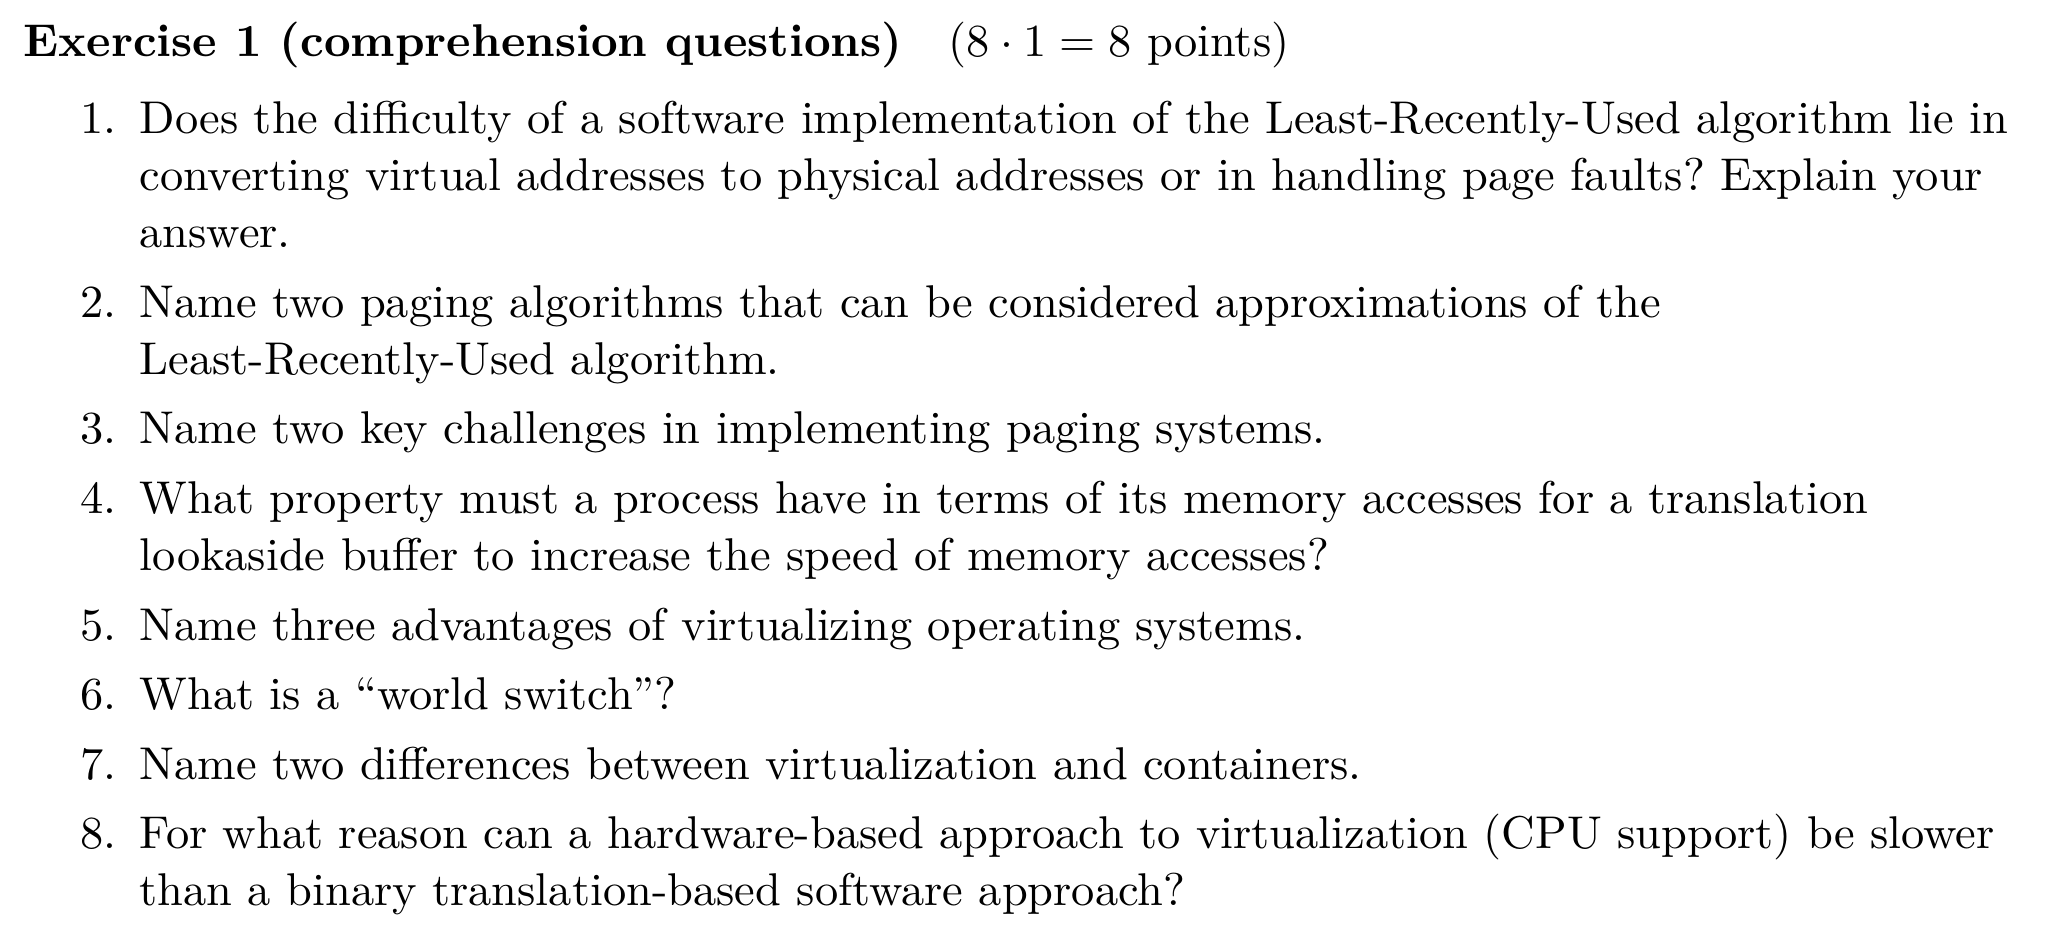
\includegraphics[keepaspectratio, width=\textwidth, height=\textheight-2\baselineskip-2\baselineskip]{img/ex6_100.png} \\
        \end{figure}
        \begin{itemize}
         \item All in the book, later part of paging and virtualization (chapter 7)
         \item Virtualization vs. containers: VirtualBox vs. Docker
        \end{itemize}
        \framebreak
        
  \begin{figure}
          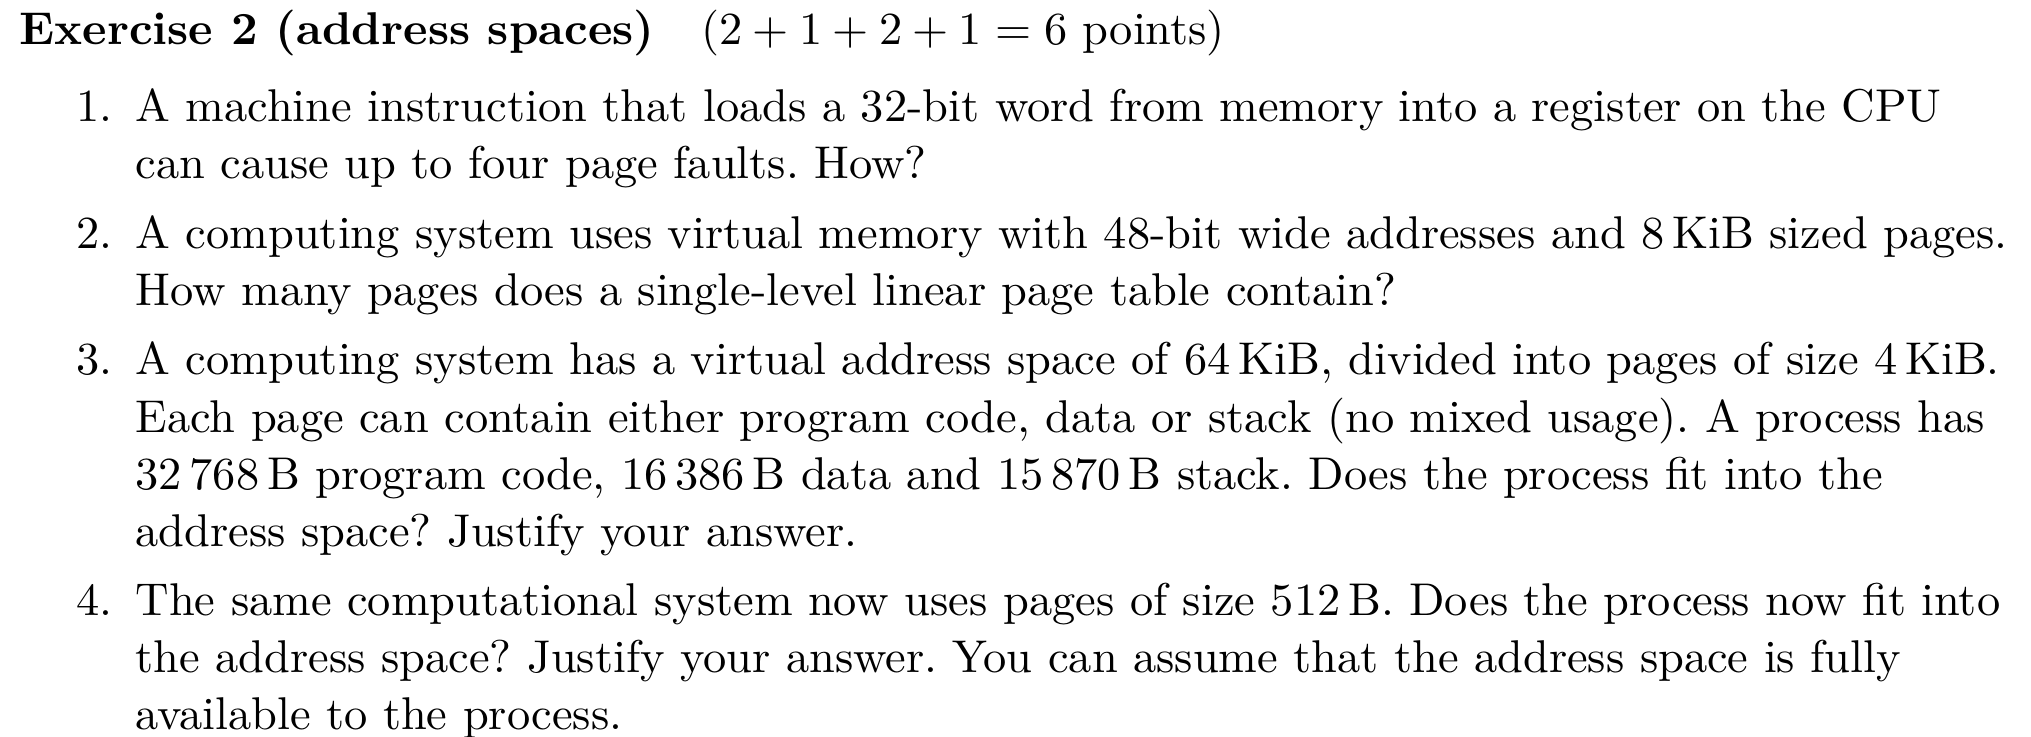
\includegraphics[keepaspectratio, width=\textwidth, height=\textheight-2\baselineskip-2\baselineskip]{img/ex6_101.png} \\
        \end{figure}
        \begin{itemize}
         \item Tanenbaum p. 236
         \item What happens if an instruction is at the boarder of two pages?
         \item Pay attention on internal fragmentation
         \end{itemize}
         
         
        \framebreak
        
         \begin{figure}
          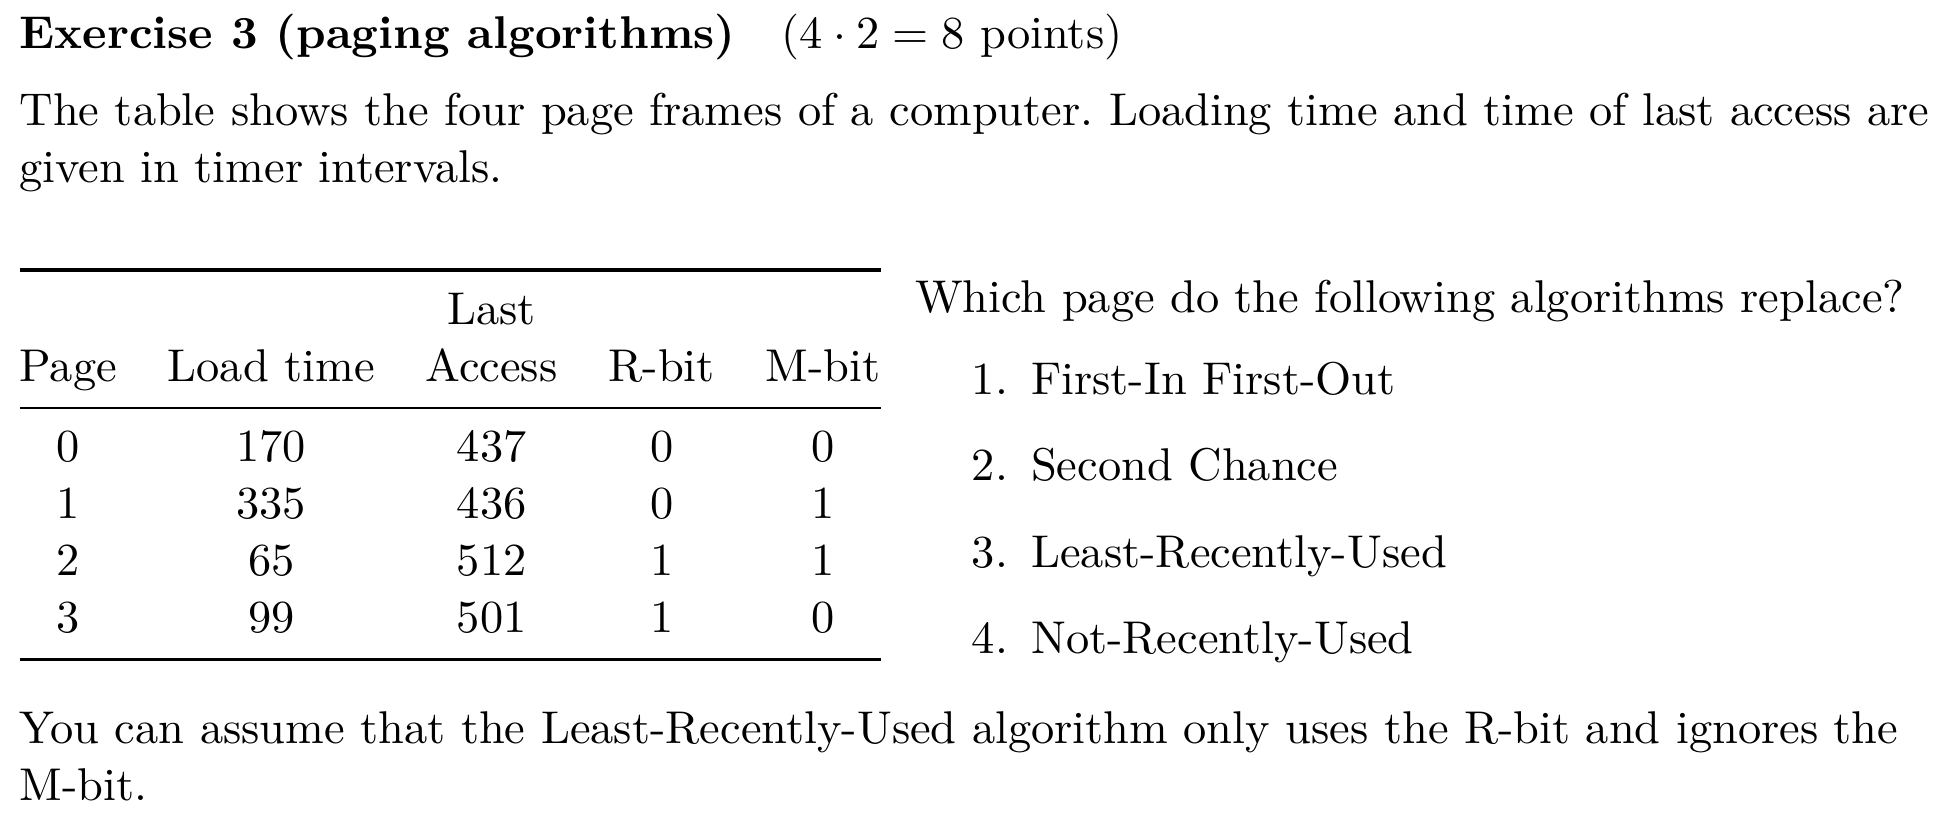
\includegraphics[keepaspectratio, width=0.8\textwidth, height=0.8\textheight-2\baselineskip-2\baselineskip]{img/ex6_102.png} \\
        \end{figure}
        \begin{itemize}
         \item FIFO depends on loading time
         \item second chance on R-bit and loading time
         \item LRU on Access time
         \item NRU on R and M bit.
        \end{itemize}
        \framebreak 
        
         \begin{figure}
          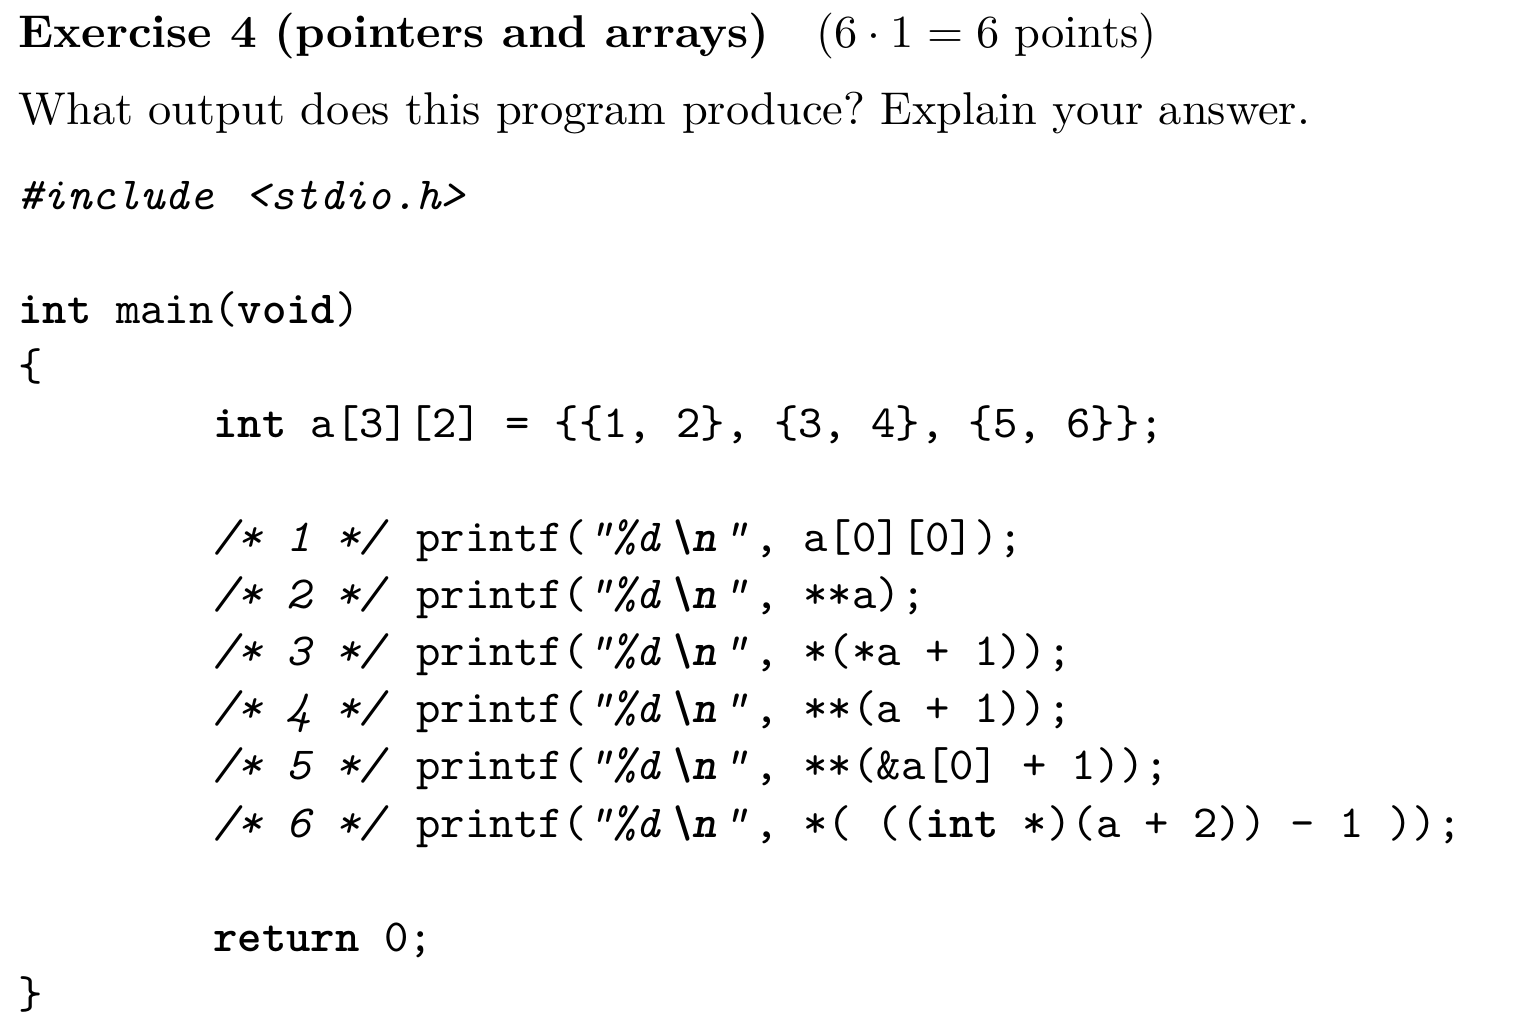
\includegraphics[keepaspectratio, width=\textwidth, height=\textheight]{img/ex6_103.png} \\
        \end{figure}
        \framebreak
        \begin{itemize}
        \item Print it and make sense of it
        \item remember that increments with pointers: +1 might also mean +4 bytes or + subarray size.
        \end{itemize}
        \framebreak 
        
        \begin{figure}
          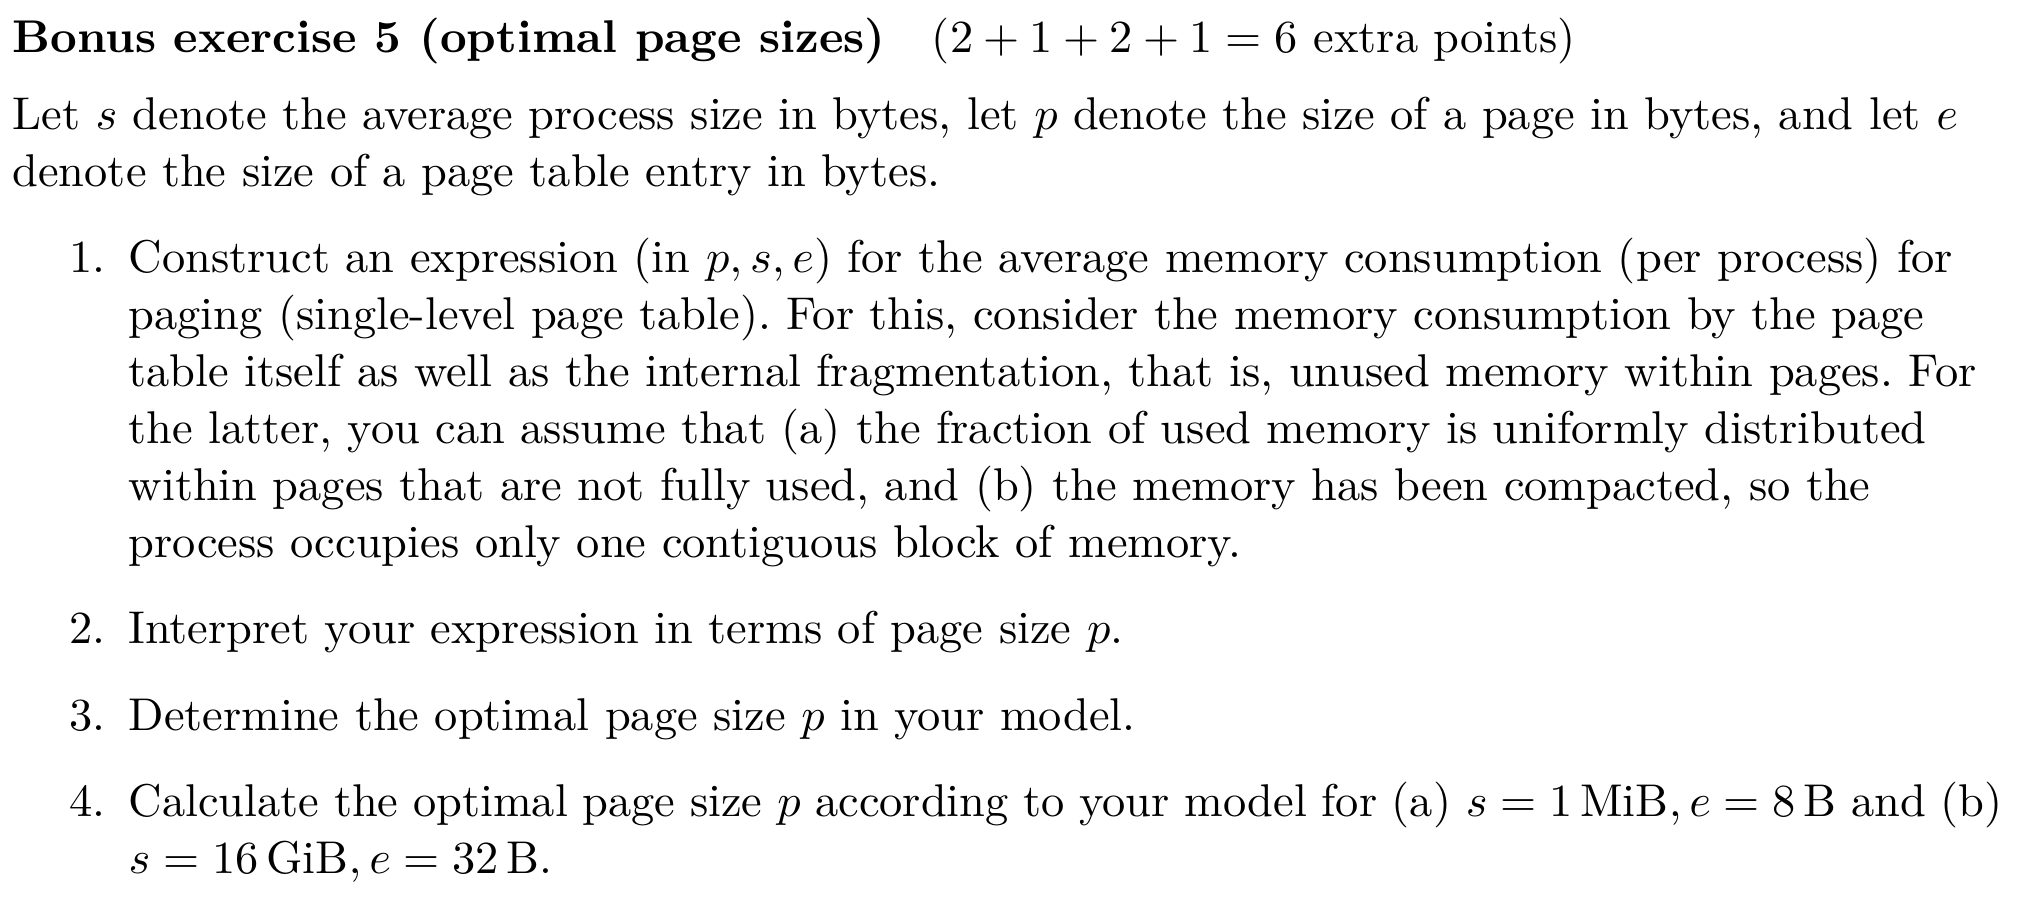
\includegraphics[keepaspectratio, width=\textwidth, height=\textheight-2\baselineskip]{img/ex6_104.png} \\
        \end{figure}
        \begin{itemize}
         \item Tanenbaum p. 226/227
        \end{itemize}
\end{frame}

\section{References}
    \begin{frame}[allowframebreaks]
      \frametitle{References}
      \begin{tiny}
      \nocite{*}
      \printbibliography
      \end{tiny}
    \end{frame}


\end{document}
 
